\documentclass[10pt]{article}
\usepackage[usenames]{color} %used for font color
\usepackage{amssymb} %maths
\usepackage{amsmath} %maths
\usepackage[utf8]{inputenc} %useful to type directly diacritic characters
\begin{document}
\begin{align*}\documentclass[10pt]{article}
\usepackage[usenames]{color} %used for font color
\usepackage{amssymb} %maths
\usepackage{amsmath} %maths
\usepackage[utf8]{inputenc} %useful to type directly diacritic characters

\usepackage{geometry}
\usepackage{graphicx}
\usepackage{listings}
\graphicspath{ {images/} }
\usepackage{pgfplots}
\pgfplotsset{width=9cm,compat=1.9}

\definecolor{codegreen}{rgb}{0,0.6,0}
\definecolor{codegray}{rgb}{0.5,0.5,0.5}
\definecolor{codepurple}{rgb}{0.58,0,0.82}
\definecolor{backcolour}{rgb}{0.95,0.95,0.92}

\lstdefinestyle{mystyle}{
  backgroundcolor=\color{backcolour},   commentstyle=\color{codegreen},
  keywordstyle=\color{magenta},
  numberstyle=\tiny\color{codegray},
  stringstyle=\color{codepurple},
  basicstyle=\footnotesize,
  breakatwhitespace=false,         
  breaklines=true,                 
  captionpos=b,                    
  keepspaces=true,                 
  numbers=left,                    
  numbersep=5pt,                  
  showspaces=false,                
  showstringspaces=false,
  showtabs=false,                  
  tabsize=2
}
\lstset{style=mystyle}

\title{LWR Equation Simulation}
\author{Hongbei Chen, Xin Peng}

\begin{document}

\maketitle

\section{Model presentation}
\begin{center}
\begin{tikzpicture}
\begin{axis}[
    axis lines = left,
    xlabel = $Distance(x)$,
    ylabel = {$Density(\rho)$},
]

\addplot [
    domain=0:5000, 
    samples=100, 
    color=blue,
    ]
    {1.333*10^(-5)*x + 0.067};
\addlegendentry{$\rho(t=0)$}

\end{axis}
\end{tikzpicture}

\textbf{Figure 1:} The vehicle density road system, typically the initial state
\end{center}

Our system expresses the vehicle density(number of vehicles per meter) on a 5000-meter-long road. This quantity varies with space$(x)$ and time$(t)$, and we use $\rho(x,t)$ to denote it. In this case, we use the $Lighthill-Whitham-Richards(LWR)$ PDE to study the system. To observe the change of vehicle density on different spaces with time going by, we set the initial density(when t=0) of the road as shown in the Figure 1.\par
In order to quantify the evolution of the density of vehicles on the road, we use a mass balance for a small control volume of length $dx$ in the road. 
Following Figure 2, we have four terms in the balance:\par
1) $\rho(x,t)dx$ number of vehicles in the control volume $[x,x+dx]$ at $t$\par
2) $\rho(x,t+dt)dx$ number of vehicles in the control volume $[x,x+dx]$ at $t+dt$\par
3) $q(\rho(x,t))dt$ number of vehicles entering the control volume $[x,x+dx]$ between $t$ and $t+dt$ through $x$\par
4) $q(\rho(x+dx,t))dt$ number of vehicles entering the control volume $[x,x+dx]$ between $t$ and $t+dt$ through $x+dx$
\begin{center}
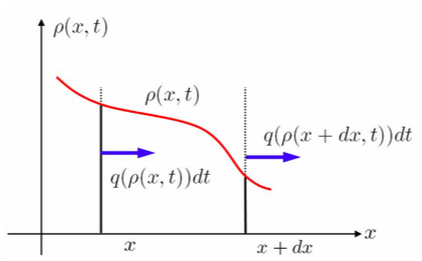
\includegraphics[scale=0.6]{fig2.png}\par
\textbf{Figure 2:} Illustration of the mass balance for the control volume $[x,x+dx]$
\end{center}
Equating the four terms in the balance, we obtain:\par
\begin{equation}\label{eq:1}
(\rho(x,t+dt)-\rho(x,t))dx = (q\rho(x,t))-q\rho(x+dx,t)))dt
\end{equation}
Dividing by $dt$ and $dx$, and taking the limit as $dt\rightarrow0$ and $dx\rightarrow0$, we obtain:\par
\begin{equation}\label{eq:2}
\frac{\partial \rho(x,t)}{\partial t}+\frac{\partial (q(\rho(x,t)))}{\partial x}=0
\end{equation}
This PDE can alternatively be rewritten as:\par
\begin{equation}\label{eq:3}
\frac{\partial \rho(x,t)}{\partial t}+q{}'(\rho(x,t))\frac{\partial (\rho(x,t))}{\partial x}=0
\end{equation}
\begin{center}
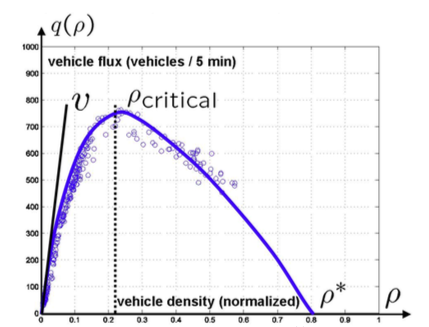
\includegraphics[scale=0.6]{fig3.png}\par
\textbf{Figure 3:} Greenshield model
\end{center}\par
$Greenshield$ $Model$ is an empirical measurement of the phenomenological law q with the density $\rho$ as shown in figure 3. Each of the dots is one measurement. The solid curve is a fit of the measurement. As can be seen, for small vehicle densities, the flux function increases almost linearly with the density (slope v). It reaches a maximum for a critical density, called $ \rho_{critical}$. For higher densities, it decreases until it finally reaches zero for a density $\rho^{*}$ called jam density.\par
According to figure 3, $Greenshield$ $flux$ $function$ is given by:
\begin{equation}\label{eq:4}
q(\rho)=v\rho(1-\frac{\rho}{\rho^{*}})
\end{equation}
where $\rho^{*}$ is the $jam$ $density$ and $v$ is the $free$ $flow$ $velocity$.\par
Combine equation (3) and (4), we get the final equation for our modeling:
\begin{equation}\label{eq:5}
\frac{\partial \rho(x,t)}{\partial t}+v(1-\frac{2\rho(x,t)}{\rho^{*}})\frac{\partial \rho(x,t)}{\partial x}=0
\end{equation}

\vspace{5mm}
\section{Implementation}

\begin{lstlisting}[language=Python, caption=Python Code]
import numpy as np
import matplotlib.pyplot as plt
from mpl_toolkits.mplot3d import Axes3D

"""
Data structure creation and initialisation
"""
# Global parameters
T_final=3600 # time duration
N_t=500 # number of time steps: the time step value dt is computed later
X_final=5000 # road length
N_x=100 # number of space steps: the space step value dx is computed later
rho0=0.2 #jam density in Greenshield flux function(number of vehicles/m)
v0=15 #free flow velocity(m/s)

# structures for visualization and computation of time/space steps
T,dt=np.linspace(0,T_final,num=N_t,endpoint=True,retstep=True)
X,dx=np.linspace(0,X_final,num=N_x,endpoint=True,retstep=True)
#set the range and sample number of time(T)–[0,3600]seconds in every 7.2 seconds
#set the range and sample number of distance(X)–[0,5000]meters in every 50 meters
print("dx = ",dx,"  dt = ",dt)

# structure for simulation: density as a function of space and time
rho = np.zeros((N_x,N_t))
# initialization of the density at time 0 with a continuous function
for x in range(int(N_x/2)):
    rho[x][0] = rho0/3+rho0*x/N_x/3 # from rho0/3 to rho0/2
for x in range(int(N_x/2),N_x):
    # rho[x][0] = rho0/3+rho0*x/N_x/3 # from rho0/2 to rho0*2/3
    rho[x][0] = rho0/3+rho0*x/N_x/3
print("t = 0")
plt.plot(X,rho[:,0])
plt.show()#plot the density in the range of x at t=0

    
"""
Start the main simulation loop
Note that the naive Euler integration scheme is ALWAYS numerically unstable
Learn about Von Neumann stability analysis
And use the simple (stable) Lax scheme
But stability needs the Courant Friedrichs Levy condition to be verified
Trick: if unstable, decrease value of dt
"""
for t in range(N_t-1): # at timestep t, compute rho at t+1
    for x in range(1,N_x-1):
        #calculate density at t+1 on i based on density at t on i and i+1
        dr = v0*dt/dx*(2*rho[x][t]/rho0-1)*(rho[x+1][t]-rho[x-1][t])/2
        r = (rho[x-1][t]+rho[x+1][t])/2 + dr #this is Lax Scheme
        rho[x][t+1] = r
    # for x==N_x, we take the derivative backward
    x = 0
    dr = v0*dt/dx*(2*rho[x][t]/rho0-1)*(rho[x+1][t]-rho[x][t])
    r = (rho[x][t]+rho[x+1][t])/2 + dr
    rho[x][t+1] = r
    x = N_x-1
    dr = v0*dt/dx*(2*rho[x][t]/rho0-1)*(rho[x][t]-rho[x-1][t])
    r = (rho[x][t]+rho[x-1][t])/2 + dr
    rho[x][t+1] = r
    if((t+1)%int(N_t/5)==int(N_t/5)-1):
        print("t = ",7.2*t)
        plt.plot(X,rho[:,t])
        plt.show()#plot the density in the range of x at t=705.6,1425.6,2145.6,2865.6,3585.6
    
        
X,T = np.meshgrid(X,T)
Z = rho.reshape(X.shape)

fig=plt.figure()
ax=Axes3D(fig)
ax.plot_surface(X,T,Z, rstride=1, cstride=1, cmap='rainbow')
plt.show()#plot the 3d figure
\end{lstlisting}
The most important part to determine stability of the system lies in line 47 and 48 in the Listing 1. A stable system would have the same code in Listing 1 which is:
\begin{lstlisting}[language=Python, caption=Stable Code]
dr = v0*dt/dx*(2*rho[x][t]/rho0-1)*(rho[x+1][t]-rho[x-1][t])/2
r = (rho[x-1][t]+rho[x+1][t])/2 + dr
\end{lstlisting}
Whereas an unstable system would have the below code to replace the stable one:
\begin{lstlisting}[language=Python, caption=Unstable Code]
 dr = v0*dt/dx*(2*rho[x][t]/rho0-1)*(rho[x+1][t]-rho[x][t])
 r = rho[x][t] + dr
\end{lstlisting}
The stable one uses $Lax-Friedrichs$ method, a numerial method for the solution of hyperbolic partial differential equations based on finite differences. Whereas the unstable one uses $Euler$ method, a first order numerical procedure for solving ordinary differential equations with a given initial value.\par
To understand the difference between these two methods intuitively, we will take the $Advection Equation$ as an example:
\begin{equation}\label{eq:6}
\frac{\partial u}{\partial t}=-v\frac{\partial u}{\partial t}
\end{equation}
To express equation(6) with $Euler$ method, we will get:
\begin{equation}\label{eq:7}
\frac{u_{x}^{t+1}-u_{x}^{t}}{\Delta t}=-v(\frac{u_{x+1}^{t}-u_{x}^{t}}{\Delta x})
\end{equation}
Whereas to express equation(6) with $Lax-Friedrichs$ method, we will get:
\begin{equation}\label{eq:8}
\frac{u_{x}^{t+1}-\frac{1}{2}(u_{x+1}^{t}-u_{x-1}^{t})}{\Delta t}=-v(\frac{u_{x+1}^{t}-u_{x-1}^{t}}{2\Delta x})
\end{equation}
We can use $Von$ $Neumann$ stability analysis to check if a numerical scheme is stable without computation. In numerical analysis, $Von$ $Neumann$ is a procedure used to check the stability of finite difference schemes as applied to linear partial differential equations. The analysis is based on the $Fourier$ decomposition of numerical error. The stability of numerical schemes is closely associated with numerical error. A finite difference scheme is stable if the errors made at one time step of the calculation do not cause the errors to be magnified as the computations are continued. A neutrally stable scheme is one in which errors remain constant as the computations are carried forward. If the errors decay and eventually damp out, the numerical scheme is said to be stable. If, on the contrary, the errors grow with time the numerical scheme is said to be unstable. $Von$ $Neumann$ analysis is often used in place of a more detailed stability analysis to provide a good guess at the restrictions (if any) on the step sizes used in the scheme because of its relative simplicity.\par
In $Von$ $Neumann$ stability analysis, we assume:
\begin{equation}\label{eq:9}
u_{x}^{t}=\xi ^{t}e^{ikx\Delta x}
\end{equation}
$\xi$ is the amplication factor and $k$ is wave number. $\xi =\xi (k)$. A numerical scheme is unstable if $\left | \xi (k) \right |>1$ and is stable if $\left | \xi (k) \right |\leq 1$. \par
First we investigate $Eular$ method, from equation(7) we get:
\begin{equation}\label{eq:10}
u_{x}^{t+1}=u_{x}^{t}+\frac{v\Delta t}{\Delta x}(u_{x+1}^{t}-u_{x}^{t})
\end{equation}
Put equation(9) into (10), we get:
\begin{equation}\label{eq:11}
\xi =1+\frac{v\Delta t}{\Delta x}(exp(ik\Delta x)-1)\Rightarrow \xi =1+\frac{v\Delta t}{\Delta x}(cos(ik\Delta x)+isin(ik\Delta x)-1)
\end{equation}
We get the amplitude $\left | \xi  \right |=\sqrt{\xi \xi ^{*}}$, where $\xi ^{*}$ is the conjugate complex of $\xi$:
\begin{equation}\label{eq:12}
\left | \xi  \right |=\sqrt{[(cos(ik\Delta x)-1)\frac{v\Delta t}{\Delta x}+1]^{2}+sin^{2}(ik\Delta x)}>1
\end{equation}
which means $Eular$ method is unconditionally unstable.\par
Then we investigate $Lax-Friedrichs$ method in the same way, from equation(8) we get:
\begin{equation}\label{eq:13}
u_{x}^{t+1}=\frac{1}{2}(u_{x+1}^{t}-u_{x-1}^{t})-\frac{v\Delta t}{2\Delta x}(u_{x+1}^{t}-u_{x-1}^{t})
\end{equation}
Put equation(9) into (13), we get:
\begin{equation}\label{eq:14}
\xi =\frac{1}{2}(exp(ik\Delta x)+exp(-ik\Delta x))+\frac{v\Delta t}{2\Delta x}(exp(ik\Delta x)-exp(-ik\Delta x))\Rightarrow \xi =cos(k\Delta x)-i\frac{v\Delta t}{\Delta x}sin(k\Delta x)
\end{equation}
We get the amplitude:
\begin{equation}\label{eq:15}
\left | \xi \right |  =\sqrt{cos^{2}(k\Delta x)+(\frac{v\Delta t}{\Delta x})^{2}sin^{2}(k\Delta x)}
\end{equation}
which means $Lax-Friedrichs$ method is conditionally stable if:
\begin{equation}\label{eq:16}
\frac{\left | v \right |\Delta t}{\Delta x}\leq 1
\end{equation}
Equation(16) is called $Courant$ $Friedrichs$ $Levy$ condition. It is a famous stability condition in numerical mathematics and is valid for many physical applications, also in inhomogenous nonlinear cases like Hydrodynamics (with v as sound speed), MHD (with v as Alfven velocity), etc.
\vspace{5mm}
\section{Results}
For the stable code, we get final plot like this:
\begin{center}
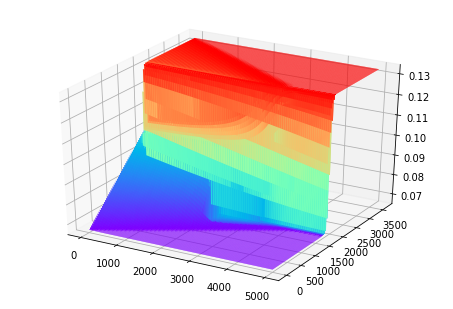
\includegraphics[scale=1]{plot1.png}\par
\textbf{Figure 4:} Final plot for stable code
\end{center}\par
And the density plot in the range of x at t=705.6,1425.6,2145.6,2865.6,3585.6 respectively:
\begin{center}
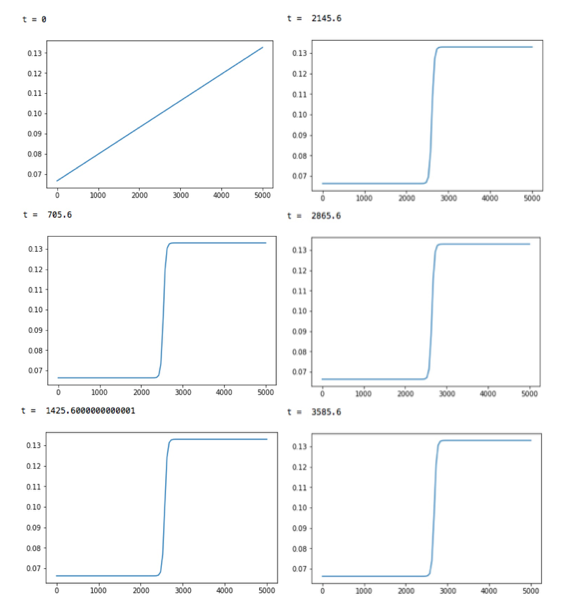
\includegraphics[scale=0.8]{plot2.png}\par
\textbf{Figure 5:} Density plot in the range of x for stable code
\end{center}\par
For the unstable code, we get final plot like this:
\begin{center}
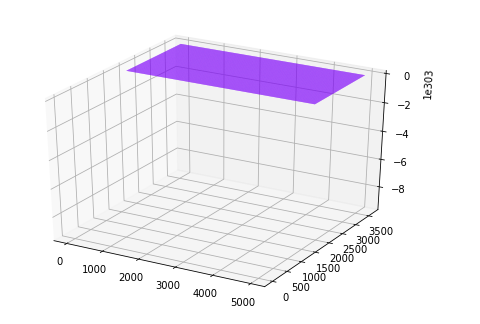
\includegraphics[scale=1]{plot3.png}\par
\textbf{Figure 6:} Final plot for unstable code
\end{center}\par
And the density plot in the range of x at t=705.6,1425.6,2145.6,2865.6,3585.6 respectively:
\begin{center}
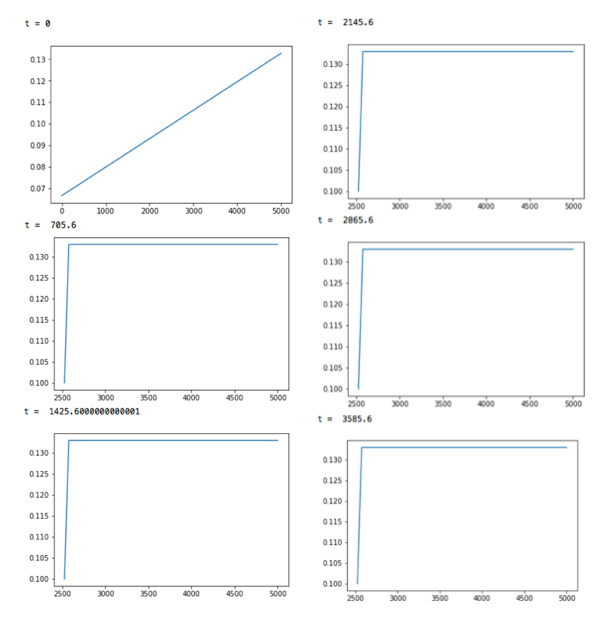
\includegraphics[scale=0.8]{plot4.png}\par
\textbf{Figure 7:} Density plot in the range of x for unstable code
\end{center}\par
\section{Interpretation}
As we can see from the Result part, we can get reasonable outputs from the stable code using $Lax-Friedrichs$ method. We understand that based on $LWR$ $PDE$ and $Greenshield$ $Model$, we will get a shock wave in the middle of the road if we start with linearly increasing density on the road at time zero. \par
However, when it comes to the unstable code using $Eular$ method, we get false outputs which make no sense. The error in each step tends to accumulate to infinite, and make the density far beyond the reasonable range.
\section{Conclusion}
From this project, we learn the $LWR$ $PDE$ and $Greenshield$ $Model$ and understand the physical meaning behind them. We learn how to describe a system and present a model. We also learn how to implement a model and do simulation with Python. And most importantly, we have realized the significance of numerical stability when doing such kind of modeling.\par
With the development of the code with $Lax-Friedrichs$ method instead of $Eular$ method, everything is aligned well in theory and practice.\par
As for the difficulty, it would be not realizing the numerical stability issue at the very beginning. Once the problem was solved, everything went out smoothly.

\medskip
\end{document}\end{align*}
\end{document}